\chapter{Описание стенда и подготовка}
\label{ch:stand}

\section{Конфигурация виртуального стенда}

Виртуальная машина \texttt{gateway} — Ubuntu~20.04.5~LTS (VirtualBox),
два сетевых адаптера:
\begin{itemize}
  \item \textbf{Адаптер~1} (\texttt{enp0s3}) — тип \textit{NAT}: выход в интернет,
        IP \texttt{10.0.2.15/24}, шлюз \texttt{10.0.2.2};
  \item \textbf{Адаптер~2} (\texttt{enp0s8}) — тип \textit{Internal Network}:
        LAN-сегмент, IP \texttt{192.168.\cfgLabStudentN.1/24}.
\end{itemize}

Виртуальная машина \texttt{Desktop} — Ubuntu~20.04.5~Desktop:
\begin{itemize}
  \item \textbf{Адаптер~1} (\texttt{enp0s3}) — тип \textit{Internal Network},
        IP получает по DHCP от gateway.
\end{itemize}

К началу лаб.~работы~\cfgLabNumber{} на \texttt{gateway} уже настроены:
маршрутизация (\texttt{ip\_forward} + iptables MASQUERADE) и DHCP-сервер
\texttt{isc-dhcp-server} (лаб.~работа~4).

% — Скриншот: настройки ВМ gateway в VirtualBox (вкладки Система, Сеть) —
\begin{figure}[h]
  \centering
  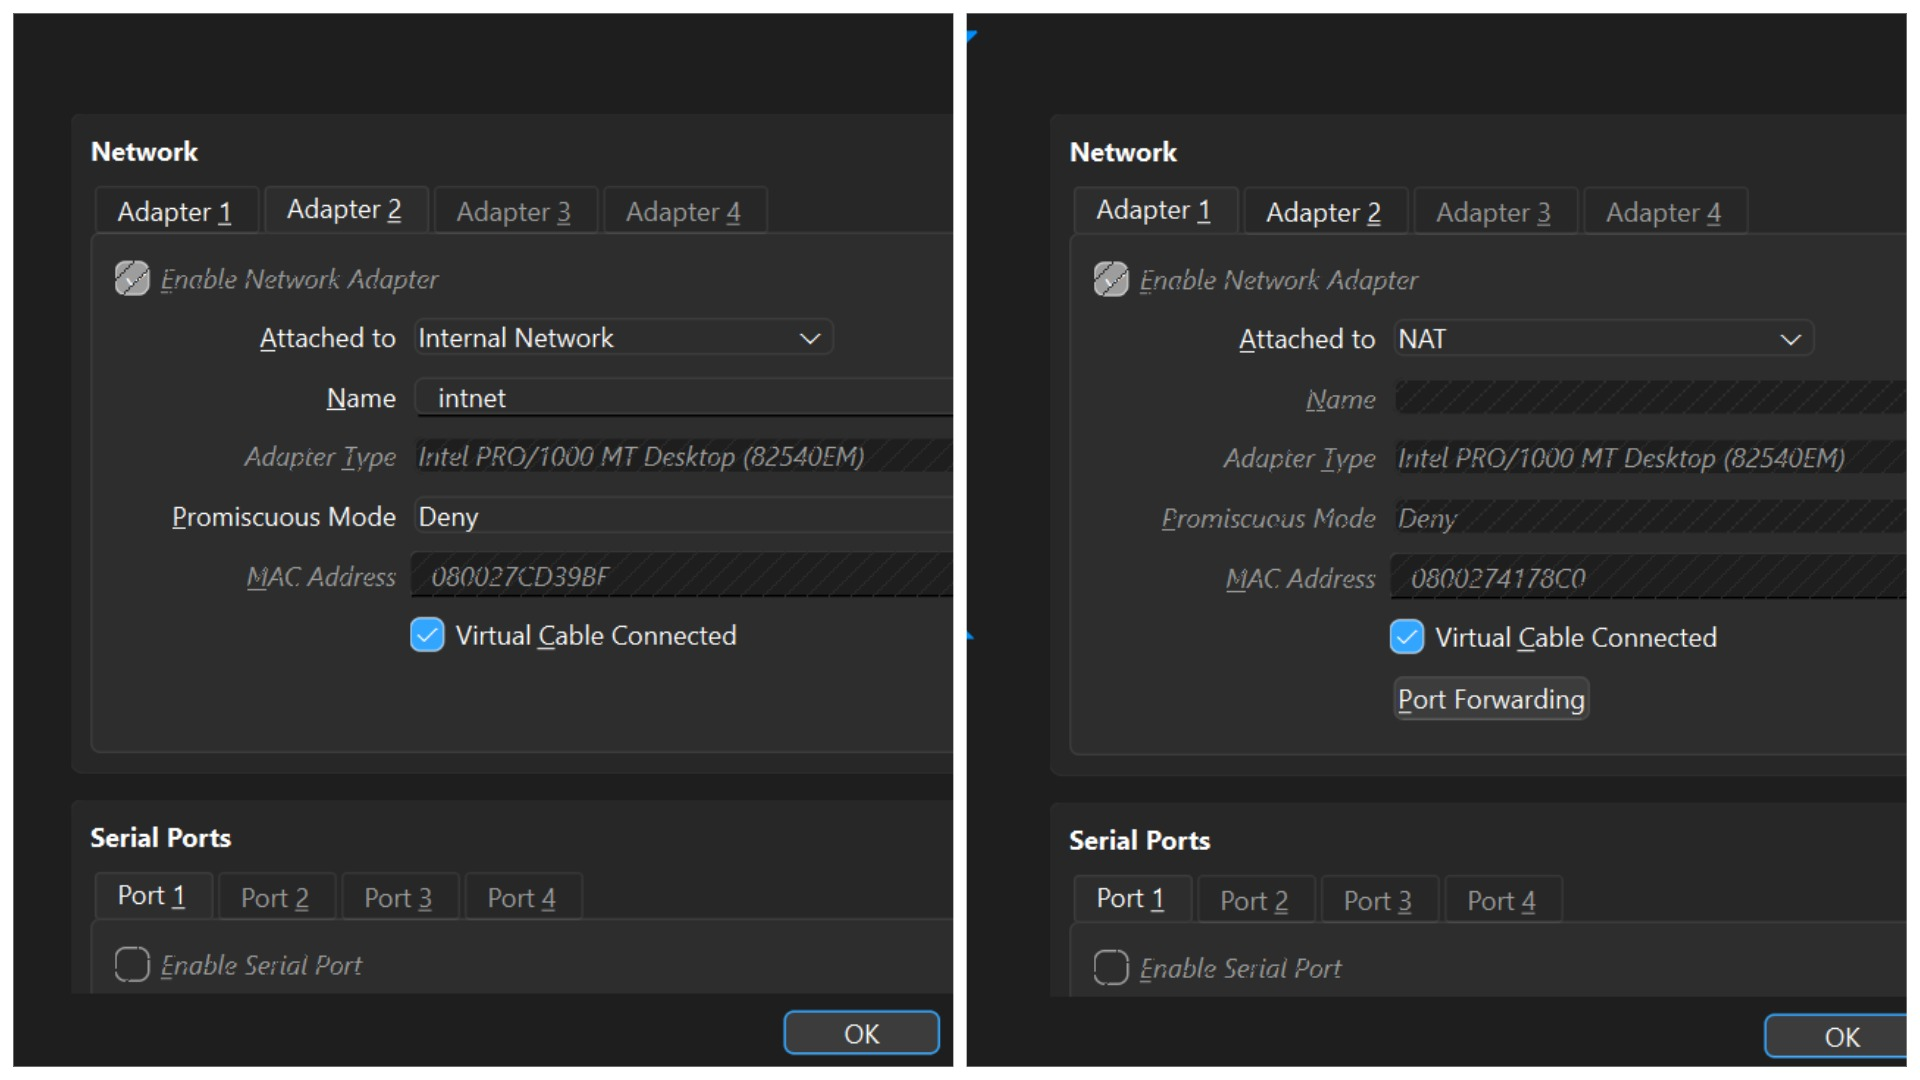
\includegraphics[width=0.85\textwidth]{img/01_vbox_gateway_settings.jpg}
    \caption{Настройки ВМ gateway — адаптеры в VirtualBox}
  \label{fig:vbox_gateway}
\end{figure}

\section{Назначение имени хоста}

По условию задания имя сервера задаётся командой
\texttt{hostnamectl set-hostname}. Формат имени: \texttt{SERVERHOSTNAME}.

\begin{lstlisting}
hostnamectl set-hostname SERVERHOSTNAME
nano /etc/hosts
\end{lstlisting}

В \texttt{/etc/hosts} добавить строку:
\begin{lstlisting}
127.0.1.1  SERVERHOSTNAME
\end{lstlisting}

% — Скриншот: nano /etc/hosts с добавленной строкой —
\begin{figure}[h]
  \centering
  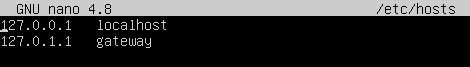
\includegraphics[width=0.85\textwidth]{img/02_etc_hosts}
  \caption{Файл \texttt{/etc/hosts} с прописанным hostname}
  \label{fig:hosts}
\end{figure}

\section{Удаление DNS DNAT-правил из лаб.~работы~4}

В лаб.~работе~4 DNS-трафик перенаправлялся на Google \texttt{8.8.8.8}.
Для использования собственного BIND9 эти правила необходимо удалить:

\begin{lstlisting}
nano /etc/iptables/rules.v4
\end{lstlisting}

Удалить строки:
\begin{lstlisting}
-A PREROUTING -i enp0s8 -p tcp -m tcp --dport 53 -j DNAT --to-destination 8.8.8.8:53
-A PREROUTING -i enp0s8 -p udp -m udp --dport 53 -j DNAT --to-destination 8.8.8.8:53
\end{lstlisting}

% — Скриншот: nano /etc/iptables/rules.v4 (строки DNAT удалены) —
\begin{figure}[h]
  \centering
  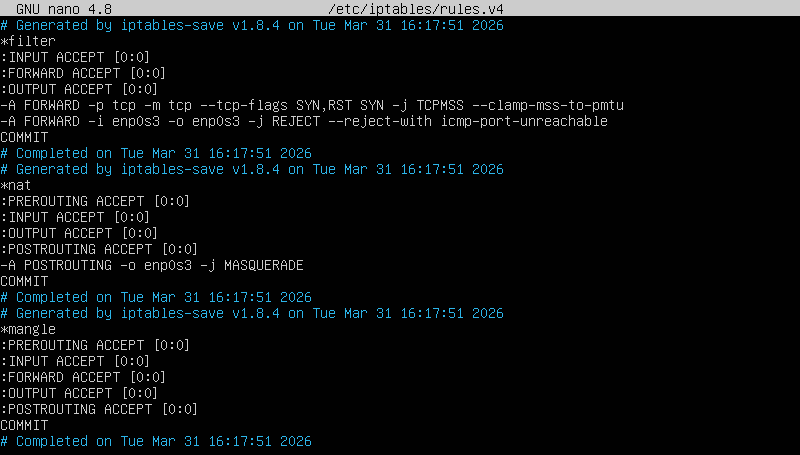
\includegraphics[width=0.85\textwidth]{img/03_iptables_rules}
  \caption{Файл \texttt{rules.v4} — правила DNAT DNS удалены}
  \label{fig:iptables}
\end{figure}

Перезагрузка:
\begin{lstlisting}
reboot
\end{lstlisting}

\section{Установка BIND9 и утилит}

\begin{lstlisting}
apt-get update
apt install bind9 dnsutils
\end{lstlisting}

% — Скриншот: вывод apt install bind9 dnsutils (завершение установки) —
\begin{figure}[h]
  \centering
  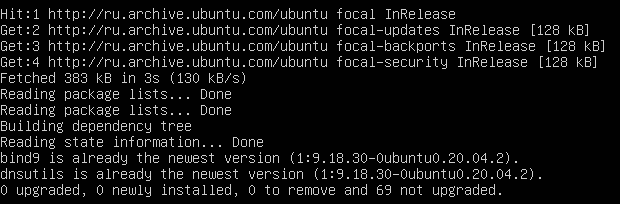
\includegraphics[width=0.85\textwidth]{img/04_bind9_install}
  \caption{Установка пакетов \texttt{bind9} и \texttt{dnsutils}}
  \label{fig:bind9_install}
\end{figure}

\endinput
